\documentclass[11pt]{article}
\usepackage{geometry}
\usepackage[utf8]{inputenc}
\usepackage{xcolor}
\usepackage{parskip}
\usepackage{graphicx}
%\usepackage{physics}

\textwidth 16cm
\textheight 24.2cm
\topmargin -2.5cm

\newcommand{\PGR}[1]{\textcolor{blue}{#1}}

\pagestyle{empty}

\begin{document}
			

\centerline{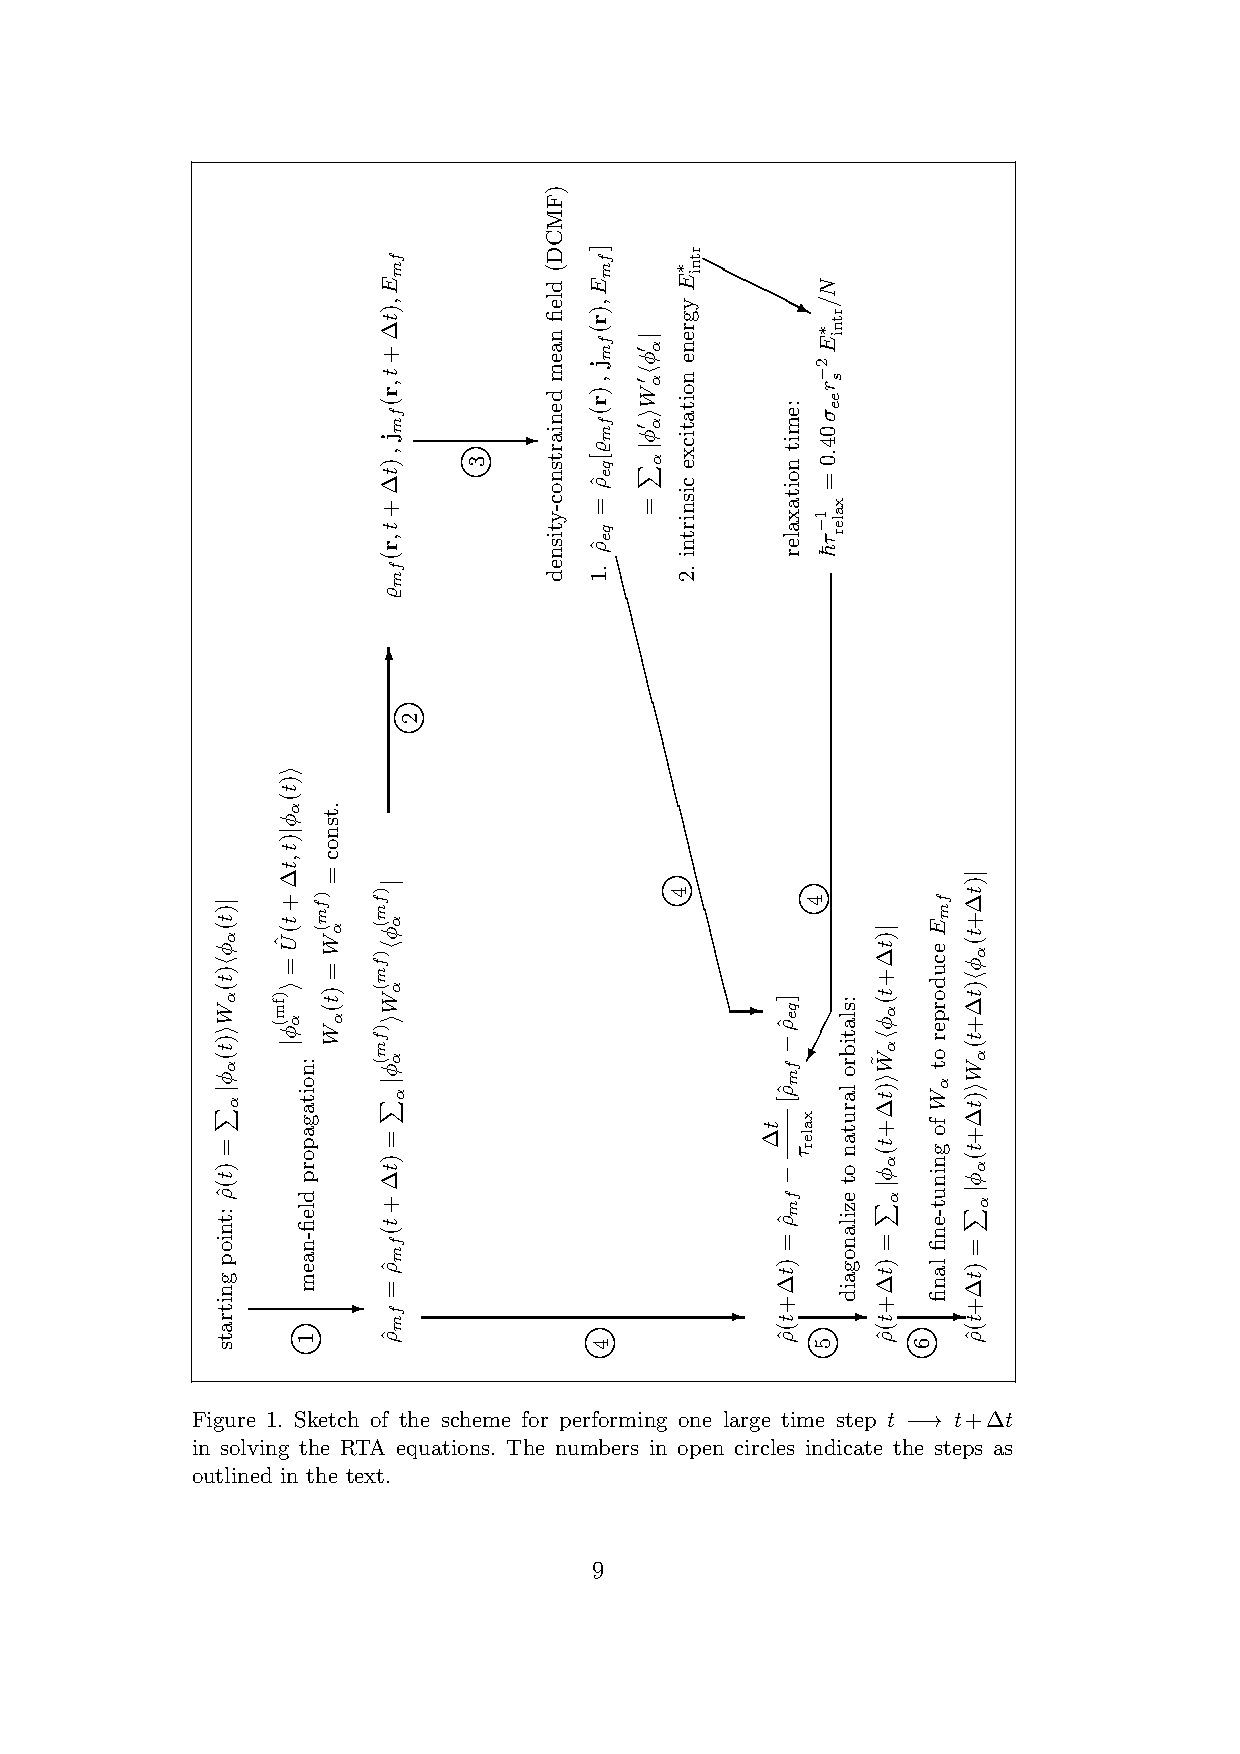
\includegraphics[height=0.9\linewidth,angle=-90]{RTA-scheme1.pdf}}


\centerline{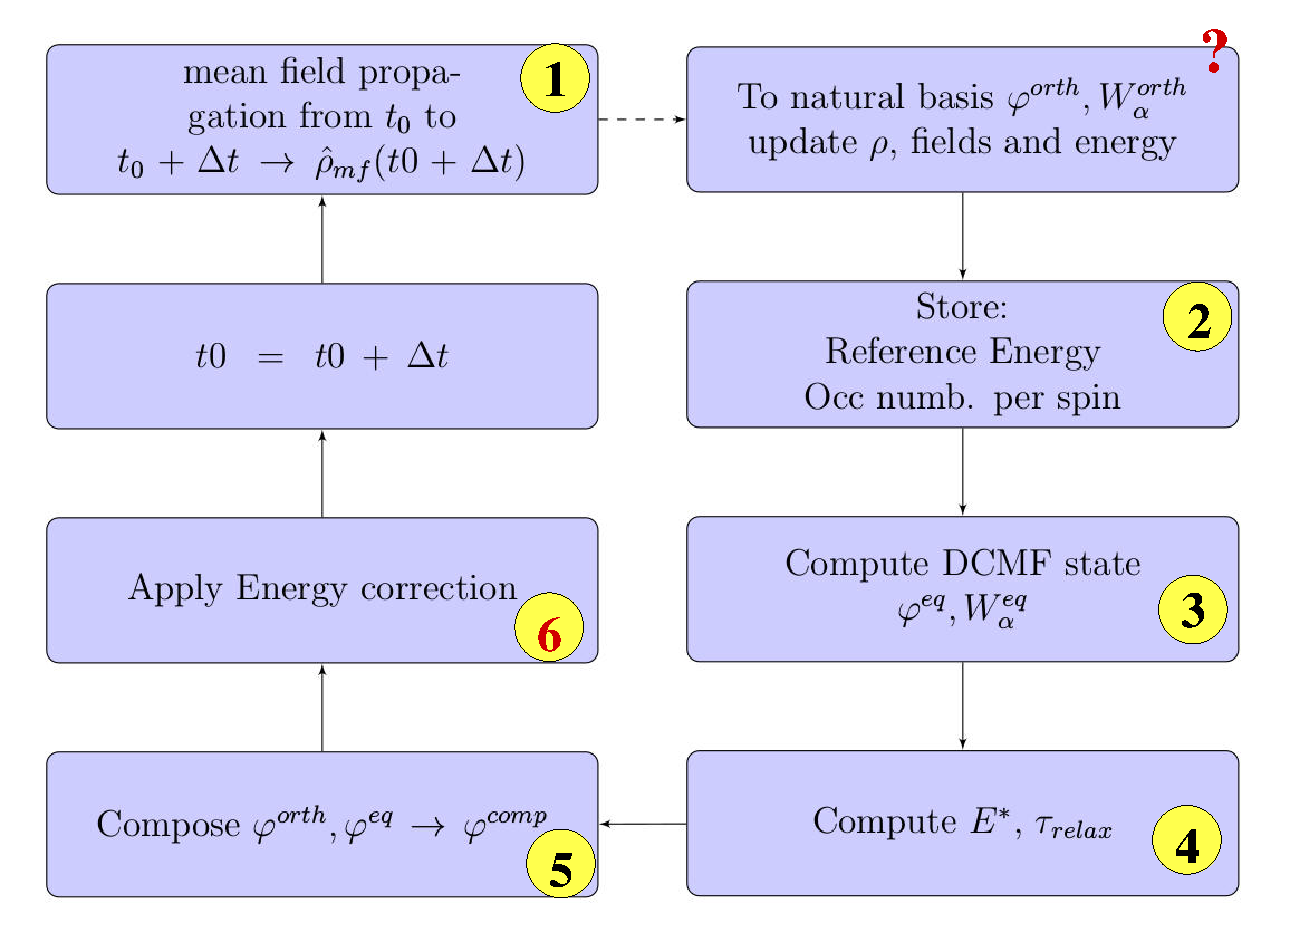
\includegraphics[width=0.8\linewidth]{RTA-scheme2b.pdf}}


The upper panel is from our Ann.Phys. paper about RTA and describes
the proceedure in the 2D code. The lower panel is from the thesis and
describes the 3D code. The numbers in the lower panels correspond to
the numbers in the upper panel.
The difference lies in the right upper of the
3D scheme. The result of TDLDA propagation is transformed to natural
oorbitals before starting DCMF and after step 5 mixing DCMF and TDLDA
one needs anothers transformation to new natural orbitals. This is not
indicated in the lower panel. Questions: First, what is the advantage of
transforming to natrual orbitals sop early, and second, are new
natural orbitals computed afters step 5?

	
\end{document}
